\documentclass[twocolumn,aps,pre,amsmath,amssymb,floatfix,longbibliography]{revtex4-1}
\usepackage{graphicx}
\usepackage{dcolumn}
\usepackage{bm}
\usepackage{amsfonts}
\usepackage{xcolor,tabu}
\usepackage{multirow}
\usepackage{amsthm}
\usepackage{textcomp}
\usepackage{tikz}
\usepackage[colorlinks=true,
            linkcolor=blue,
            urlcolor=blue,
            citecolor=blue]{hyperref}
\hypersetup{bookmarksopen=true}
\usepackage{xr}
\externaldocument{correlation_SI}


\begin{document}
\title{Density Correlations and Fluctuations in Bacterial Suspensions}

\author{Zhengyang Liu}
%\email{liux3141@umn.edu}
\author{Wei Zeng}
\author{Xiaolei Ma}
\author{Xiang Cheng}


\affiliation{Department of Chemical Engineering and Materials Science, University of Minnesota, Minneapolis, Minnesota 55455, USA}

\date{\today}


\begin{abstract}
Active systems, such as bacterial suspensions, exhibit strong density correlations and  fluctuations. While these phenomena at high concentration are well established, it remains unclear whether they persist or simply vanish when concentration is brought below the turbulence transition. We report simultaneous measurements on correlations and density fluctuations in \textit{E. coli} suspensions at various concentrations. We find a nontrivial density fluctuation below the turbulence transition, which is characterized by a gradual increase with concentration, in contrast to the sudden increase of density correlations. Our kinetics study reveals the underlying mechanisms of the density fluctuations.
\end{abstract}



\maketitle
\section{Introduction}

Bacterial suspensions are premier example of active matter. Being constantly driven out of equilibrium, they exhibit anomalous properties drastically different from systems in equilibium, including enhanced diffusivity, reduced viscosity and giant number fluctuations. While the anomalous diffusion and rheology have only been demonstrated in microscopic scale, the giant number fluctuations are predicted to be more universal across various length scales. Indeed, such fluctuations have been observed in bird flocks \cite{Ballerini1232}, fish schools \cite{Ward6948}, shaking granules \cite{Narayan105}, bacteria on agar gels \cite{Zhang13626} and active actin filaments \cite{Schaller4488}. Such universality makes giant number fluctuations a popular topic in active matter.

Despite the extensive efforts to model and measure giant number fluctuations in a variety of systems, some physical aspects of the phenomenon remain unclear. We seek to understand the phenomenon better by experimenting with \textit{E. coli} bacteria.

First, how the fluctuation depends on the crowdedness of "swimmers" is not elucidated. Although it has been shown that the fluctuation is stronger in crowded environment \cite{PhysRevE.95.020601, Zhang13626}, most experiments to date have assumed two regimes: low concentration and high concentration. Within each concentration regime, fluctuations are identical. In other words, at high concentrations, number fluctuations are always of the same magnitude, while at low concentration, giant number fluctuations become absent. The simple picture was great for appreciating the macroscopic concsequences of collective motions. However, a lack of detailed measurements on concentration dependence hindered the discovery of the microscopic origin of giant number fluctuations. The dependence of giant number fluctuations on concentrations is subtle and has been hinted by experiment with bacteria on 2-D surface\cite{Zhang13626}. In this paper, we present a more systematic measurement on concentration dependence, which points to the microscopic origin of giant number fluctuations.

Second, how the magnitude of giant number fluctuation evolves has never been measured. And this is due to the fact that the most widely used experimental platform - bacterial suspensions - suffers from a lack of control over the motility of bacteria. To overcome this limitation, we use a light-controlled \textit{E. coli} strain, whose primary energy source is light, so that the swimming speed can be instantaneously and precisely controlled. This evolution can reveal the intrinsic time scale of an active system. More importantly, comparisons can be made with the evolution of other quantities \cite{Peng2020}, such as flow order and flow energy, to reveal the underlying mechanisms of giant number fluctuations.

Third, while theories predict that giant number fluctuations depend on dimensionality \cite{PhysRevLett.75.4326, PhysRevE.58.4828, EPL2003, doi:10.1146/annurev-conmatphys-031119-050752}, all simulations and experiments so far have been done in 2-dimensional space \cite{PhysRevE.77.046113, PhysRevLett.123.218001, Schaller4488, PhysRevE.95.020601}. This work examines giant number fluctuations in 3-D space experimentally for the first time, and also compare the result with 2-D space under similar experimental setting. Thus, this work provides a good platform for testing existing theories.

Measuring instantaneous local bacterial concentration is required in order to quantify the magnitude of giant number fluctuations. Yet, it is challenging. Inspired by earlier experimental works, where fluorescence intensity serve as indicators of local concentration \cite{Schaller4488}, we come up with the idea that light transmission - the natural information in bright field microscope images - could also indicate local concentrations. This idea is an extension of Beer-Lampert law, where the attenuation of light and particle concentration are related. Such principle is used in the spectrophotometer, with which we measure the concentration of bacterial suspensions. Similar idea, where fluctuations in image intensity is proportional to fluctuations in concentration, has been assumed in another work \cite{PhysRevLett.106.018101}. Here, we experimentally verify the assumption, showing that concentration and image intensity follow a nearly linear relationship (\textcolor{red}{Fig.~S1}). The idea gets more concrete if we look at Fig.~\ref{fig:1}c - a snapshot of dense bacterial suspensions - where giant number fluctuations lead to strong alternation of dark and bright region. In contrast, in a dilute suspension shown in Fig.~\ref{fig:1}a, where giant number fluctuations are absent, such intensity alternation is not observed.

Since local concentration measurements are made possible by the idea of using image intensity as indicator, we are able to fill in the missing pieces of the knowledge about giant number fluctuations in 3-D bacterial suspensions. Our most important finding is that: motility induced fluid flow drives the giant number fluctuations, and the strength of flow is the key parameter that governs the magnitude of number fluctuations. We also show that fluid convection is the microscopic origin of local number fluctuations, in consistency with then main finding. Moreover, we show that in a confined quasi-2D geometry, giant number fluctuation gets weaker, which again confirms the key finding, because motility induced flow is largely suppressed due to the closely spaced no-slip boundaries. This work presents systematic measurements on giant number fluctuation phenomenon, providing a good platform for testing and developing active matter theories. By relating microscopic dynamics and macroscopic properties, our finding also shed new light on emergent collective behaviors in active matter.
%
% Here, we show that \textit{E. coli} suspensions at concentrations above 60 n$_0$ shows giant number fluctuations with $\Delta N \varpropto N^\alpha$, where $\alpha\approx0.83$, close to the predictions on dry active nematics (0.83) and dry active polar fluids(0.76). Remarkably, the scaling exponent, $\alpha$, shows a dependence on concentration below 60 n$_0$, which does not vanish at 20 n$_0$ (below the active turbulence transition, 40 n$_0$). This nontrivial dependence on concentrations below the active turbulence transition suggests that giant number fluctuations can arise without apparent collective motion (where groups much larger than individuals moving together can be identified), in consistency with a recent theoretical work \cite{PhysRevLett.119.028005}.

% This fluctuation is shown to result from topological defects in the associate flow field, where transient high density "clusters" appear and disappear.

%\begin{figure}[!]
%\begin{center}
%\includegraphics[]{}
%\caption[]{}
%\end{center}
%\end{figure}

\section{Experiment}

\subsection{Light-controlled bacteria}
We introduce a light-driven transmembrane proton pump, proteorhodopsin (PR), to wild-type \textit{E. coli} (BW25113) by transforming the bacteria with plasmid pZE-PR encoding the SAR86 $\gamma$-proteobacterial PR-variant \cite{Walter2408}. The activity of PR is directly correlated with the light intensity. Thus, we can control the swimming speed of bacteria using light of different intensities.

The bacteria are cultured at 37 \textcelsius with a shaking speed at 250 rpm for 14-16 hours in terrific broth (TB) [tryptone 1.2\% (w/w), yeast extract 2.4\% (w/w), and glycerol 0.4\% (w/w)] supplemented with 0.1 g/L ampicillin. The culture is then diluted 1: 100 (v: v) in fresh TB and grown at 30 \textcelsius for 6.5 hours. PR expression is triggered by supplementing the culture medium with 1 mM isopropyl $\beta$-D-thiogalactoside and 10 \textmu M ethanolic all-trans-retinal in the mid-log phase (3 hours after the dilution).

The bacteria are harvested by gentle centrifugation (800g for 5 min). After discarding the culture medium in the supernatant, we resuspend bacteria with dI water. The resuspended suspension is then centrifuged again at 500g for 5 min, and finally adjusted to target concentration for microscopy.

\begin{figure}[!]
\begin{center}
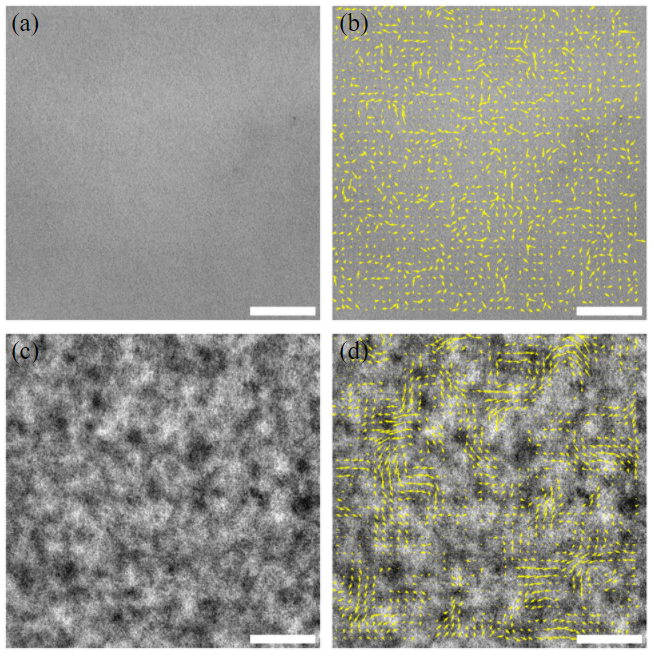
\includegraphics[width=0.45\textwidth]{GNF-figures-1-v2.png}
\caption[]{Bright-field microscopy of a bacterial suspension at 80 n$_0$ (a) and the velocity field at the instance (b). Scale bar is 100 \textmu m. (c) Relation between bacterial suspension concentrations (measured by OD600 spectrometer) and average image intensities (red squares). Error bars represent the standard deviations of pixel intensities in an image. The black dashed line is a linear fitting of the relation. }
\label{fig:1}
\end{center}
\end{figure}

\subsection{Sample preparation and microscopy}

To prepare the sample for microscopy, we put bacterial suspensions prepared from the previous step into a seal chamber made of glass slides (25 mm $\times$ 75 mm) and coverslips (18 mm $\times$ 18 mm). We first glue (Norland 81) two coverslips on a glass slide, side-by-side, leaving a 3-mm separation between the two coverslips. We then cover the 3-mm separation with another coverslip to form a "channel". Then we use pipet to inject bacterial suspensions into the channel. Finally, we seal the two ends of the channel using UV glue (Norland 76) to form a sealed chamber.

The sample bacterial suspensions are images through an inverted bright-field microscope using a 20$\times$ (NA 0.5) objective. The filed of view is 640 $\times$ 640 \textmu m$^2$ (Fig.~\ref{fig:1}a). In order to control the velocity of bacteria by light, we wait for 10 minutes after loading samples so that bacteria can deplete the disolving oxygen in the samples and stop swimming when light is switched off. Then we switch on the light to trigger the light-powered motility. We wait another 2 minutes for the collective motion to reach a steady state under the new light condition, and start to take images. All the videos are recorded at 30 frames per second using a sCMOS camera.

\subsection{Kinetics}
The growth of giant number fluctuations is imaged when we tune up the swimming speed of \textit{E. coli} by light. Videos are taken at 30 FPS for 1 minute. The light intensity is tuned from low to high at 5 seconds. Note that, to avoid a short unstable period of the light source when adjusting the voltage (\textcolor{red}{Fig.~S2}), we set the voltage fixed at high at the beginning of each experiment. In the first 5 seconds, the light source is blocked with a neutral density filter, which is then removed to achieve high light intensity.

\begin{figure}[!]
\begin{center}
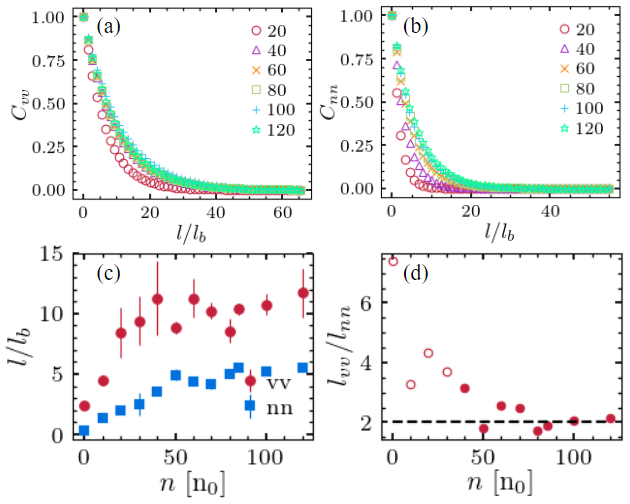
\includegraphics[width=0.5\textwidth]{GNF_figure-2-v2.PNG}
\caption[]{\textbf{Spatial correlation functions and correlation lengths.} (a, b) velocity and image intensity correlation functions, (c) velocity and image intensity correlation length (defined as $C=1/e$) and (d) ratios between the two correlation lengths at concentrations = 20, 40, 60, 80, 100 and 120 n$_0$.}
\label{fig:2}
\end{center}
\end{figure}


\begin{figure*}[!]
\begin{center}
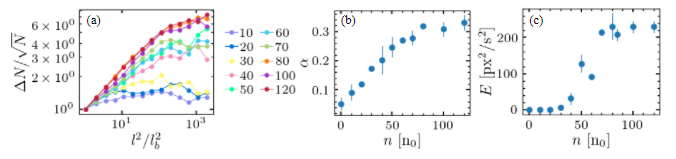
\includegraphics[width=\textwidth]{GNF-figures-3-v3.png}
\caption[]{\textbf{Concentration dependence} (a) Giant number fluctuations in bacterial suspensions at concentrations ranging from 10 to 120 n$_0$. The $\Delta N/\sqrt{N}$ is in fact $\Delta I/l$, where $I$ is the average pixel intensity of a subsystem and $l$ is the linear size of the subsystem. The $\Delta N/\sqrt{N}$ value is rescaled by the first value of each curve, so that all the curves start from $\Delta I/l=1$. (b) The scaling exponents $\alpha$ ($\Delta N \propto N^{0.5+\alpha}$) of number fluctuation curves as a function of bacterial concentrations. (c) Steady- state flow energy as a funciton of bacterial concentrations.}
\label{fig:3}
\end{center}
\end{figure*}


\subsection{Correlation analysis}

\subsubsection{Flow fields}
The flow fields are measured by Particle Image Velocimetry (PIV) analysis using openPIV package in Python \cite{openpiv} (Fig.~\ref{fig:1}b). We choose box size to be 16 \textmu m, which is much larger than a single bacterium body to enhance statistical accuracy, and smaller than the typical length scale of the collective motion of \textit{E. coli} so that the features are not smoothed out. We choose step size to be half of the box size (8 \textmu m) by convention.

\subsubsection{Concentration fields}
The concentration fields are measured directly from the image pixel intensity fields. In an attempt to calibrate the concentration-intensity relation, I fix the light intensity on microscope, and load bacterial samples of various concentrations. Then I plot the concentrations as a function of corresponding average image pixel intensities, as shown in \textcolor{red}{Fig.~S1}. This result suggests that concentration and image intensity follows approximately a linear relation, or formally:
$$ c = aI + b $$
where $c$ is bacterial concentration, $I$ is pixel intensity, $a$ and $b$ are constants. This linear relation will be used in the number fluctuation calculation in Sec.~\ref{sec:method_gnf}.
\subsubsection{Spatial correlations}

The spatial correlation of a quantity $A$ (concentration, velocity or orientation) is defined as the following:

$$ C(x, y) = \frac{\langle(A(x_0+x, y_0+y)-\bar A)(A(x_0, y_0)-\bar A) \rangle_{x_0, y_0}}{\langle(A(x_0, y_0)-\bar A)^2\rangle_{x_0, y_0}}$$

where $\langle\cdot\rangle_{x_0, y_0}$ denotes the spatial average of a quantity over all possible $x_0$'s and $y_0$'s.  $\bar A$ denotes the spatial average of $A$, i.e. $\bar A=\langle A\rangle_{x_0, y_0}$.

\subsubsection{Temporal correlations}
The temporal correlation of a quantity $B$ (concentration) is defined as the following:

$$ C(\tau) = \frac{\langle (B(t+\tau)-\bar B)(B(t)-\bar B)\rangle_t}{\langle(B(t)-\bar B)^2\rangle_t} $$

where $\langle\cdot\rangle_{t}$ denotes the spatial average of a quantity over all possible $t$'s.  $\bar B$ denotes the temporal average of $B$, i.e. $\bar B=\langle B\rangle_{t}$.

\subsubsection{Coarse-graining}
All the correlation analyses are done on coarse-grained data. On the one hand, we obtain velocity fields using PIV, which requires the image to be divided into interrogation boxes. On the other hand, the pixel size of our image is 0.33 \textmu m, which is much smaller than a \textit{E. coli} bacterium. As a result, the intensity of a single pixel may reflect the local concentrations of a suspension, but rather the structures within one bacterium body. Therefore, we divide our images into boxes of the same size as is used in PIV analysis, for the concentration field correlation analysis (and the giant number fluctuation analysis).

As discussed above, the box size needs to be larger than the size of a \textit{E. coli} bacterium. In addition, it should not be larger than the correlation length of the concentration or velocity fields, so that the correlations can still be captured after coarse-graining. We varied the box size and step size to perform PIV analysis, and it turns out that setting box size at 16 \textmu m and step size at 8 \textmu m gives reasonable results (SI figure \textcolor{red}{Fig.~S3}).

\subsection{Giant number fluctuation analysis}\label{sec:method_gnf}
Two methods have been used to quantify giant number fluctuations. One of them, which divides a frame of an image sequence into small boxes and measure the standard deviation of particle numbers in these boxes. Then the procedure is repeated over all the frames, and the average of the standard deviations gives a measure of number fluctuations of the system (Menon 2007). The other method, which also divides images into small boxes, measures the standard deviations of numbers of particles in each box over time. Then the standard deviations are averaged in space to give a measure of number fluctuations of the system (Urbach 2008). Urbach 2008 futher stated that when a system is homogeneous, where spatial and temporal correlations are small compared with the system size and experiment duration, two methods give the same result. Our experimental system, \textit{E. coli} suspensions, has a correlation length ($\sim 50$ \textmu m) much smaller than the system size ($\sim 140$ \textmu m), and is thus a spatially homogeneous system. However, since we rely on image pixel intensity to indicate the local concentrations, a slight inhomogeneity of illumination would result in a long standing concentration inhomogeneity, which is not true in reality (see \textcolor{red}{Fig.~S4}).

Therefore, we use the second method, since the illumination inhomogeneity is long standing and stable over time. We can think of it as adding a constant image to each frame, which does not affect the temporal variation calculation. We take box size ranging from 10 to 30 \textmu m, and examine the temporal variations of bacterial concentrations $\Delta N_{ij}$ in the $i^{th}$ box for each box size $l_j$. The temporal variations are then averaged in space (over $i$) to give a single value variation $\Delta N_{j}$. Then number fluctuations in the system is captured by the dependence of $\Delta N_{j}$ on $l_j$. In an equilibrium system, $\Delta N_{j}\propto l_j$ (this follows from $\Delta N_{j}\propto \sqrt{N_j}$ and $N_j\propto l_j^2$). Thus, the deviation from $\Delta N_{j}\propto l_j$ quantifies the giant number fluctuation in the system. Here, we plot $\Delta N_{j}/l_j$ as a function of $l_j^2/l_b^2$. To be consistent with the notations in literatures, we get rid of the subscript $j$, and write $l_j$ as $\sqrt{N}$. Note that the subscript $j$ denotes different choices of box sizes.


\section{Results and discussion}



\begin{figure*}[!]
\begin{center}
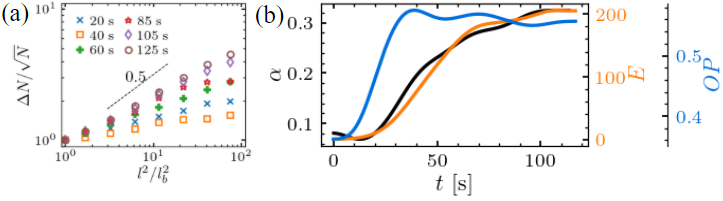
\includegraphics[width=\textwidth]{GNF_figure-4-v1.png}
\caption[]{\textbf{Evolution of giant number fluctuations at concentration $n=80$ n$_0$.} (a) Standard deviation of particle numbers $\Delta N$ scaled by the square root of the mean $\sqrt N$ as a function of subsystem size rescaled by bacterial body size $l^2/l_b^2$. Numbers in legends denotes the time from the point when bacterial motility is triggered by light (seconds). (b) The temporal evolution of the scaling exponents $\alpha$, flow energy $E$ and flow order parameter $OP$.}
\label{fig:4}
\end{center}
\end{figure*}

\begin{itemize}
\item Correlation Results
\item GNF Result
\item interplay Results
\item discussion (wave, lifetime, length scale implication, low concentration correlation, etc)
\end{itemize}

\subsection{Spatial correlations}
We analyzed the spatial correlations of flow velocity and concentration (Fig.~\ref{fig:2}a-b) of motile \textit{E. coli} suspensions at various concentrations. Both correlation lengths show a gradual increase at low concentration and saturate at high concentration (Fig.~\ref{fig:2}c). The crossover concentration of both correlation lengths are around 40-50 n$_0$, suggesting a transition from a disordered state to turbulence. The gradual increase at low concentration suggests that, even below the apparent turbulent transition, bacteria, or more generally active agents, start to move in a correlated way \cite{PhysRevLett.119.028005}. \textcolor{red}{Remarkably, we show that above the crossover concentration, the ratio between velocity correlation length and concentration correlation length converges to 2 (Fig.~\ref{fig:2}d). We have not fully understood the significance of this ratio, but it tends to suggest a close correlation between concentration and velocity field. In the following analysis of giant number fluctuations, we hope to elucidate this correlation.} Moreover, our finding suggest that spatial concentration correlation length, in addition to flow velocity correlation length\cite{Wensink14308, PhysRevLett.110.228102}, can be used to mark the transition to active turbulence.

\subsection{Giant number fluctuations}
\textbf{Concentration dependence} We measured the number fluctuations at concentrations ranging from 10 n$_0$ to 100 n$_0$. As can be seen in Fig.~\ref{fig:3}a, as concentration gets higher, the fluctuation gets stronger and deviates farther from thermal equilirium. A more quantitative description of the concentration dependence is shown in Fig.~\ref{fig:3}b, where the scaling exponents $\alpha$ extracted from Fig.~\ref{fig:3}a are plotted against concentrations. $\alpha$ gradually increases with concentrations, and plateaus above 70 n$_0$. The plateau value of $\alpha$ at high concentrations is around 0.32, close to the theoretical prediction made by Simha and Ramaswamy \cite{PhysRevLett.89.058101}. Their theory follows from a set of hydrodynamic equations of motion, and implies that the standard deviation $\Delta N$, scaled by $\sqrt N$, diverges as $N^{1/3}$. At low concentrations, $\alpha$ increases smoothly up to 70 n$_0$, different from the turbulence transition, 40-50 n$_0$, marked by the crossover of velocity and concentration correlation lengths. This difference is defying our intuition that the giant number fluctuations are always the same once turbulent state is triggered. Such difference is attributed to flow energy. In Fig.~\ref{fig:3}c, we plot the steady-state flow energy, defined as the sum of velocity squares, as a function of concentration. This esult suggest that, above 40 n$_0$, within the turbulent state, the steady-state flow energy is not constant. Instead, it shows an abrupt increase from 40 n$_0$ to 70 n$_0$, after which it plateaus. The range of flow energy increase coincides with the range of increasing of $\alpha$, implying a correlation between flow energy and magnitude of number fluctuations. This correlation will appear again and get more evident further on.

\textbf{Evolution} By virtue of the light-controlled \textit{E. coli}, we are able to image how a "dead" suspension gradually start to mix, form patterns, deviate from the thermal equilibrium and exhibit giant number fluctuations. Fig.~\ref{fig:4}a shows how standard deviation scales with the mean and how it evolves over time. Initially, the collective motion is not fully developed, and the scaling exponent $\alpha$ is low. After 100 seconds, the increase of $\alpha$ slows down. The evolution of $\alpha$ is shown in a finer temporal resolution in Fig.~\ref{fig:4}b. In addition, the flow energy and flow order parameter for the same process are plotted as well in Fig.~\ref{fig:4}b \cite{Peng2020}. High flow energy indicates that the fluid elements are moving vigorously, and high order parameter indicates that most of the flows are moving along the directions of their neighbors. When order parameter is high, the flow field appears to us as a turbulence. The order parameter initially increases, and then reaches a plateau value of 0.56 at 40 seconds. At this point, the flow already looks like turbulence, but the energy is still low. After another 60 seconds, flow energy also reaches a plateau and the flow is then exhibiting the most vigorous turbulence. Remarkably, we find that $\alpha$ and $E$ evolve almost along the same trajectory, and both reach a high plateau value at 100 seconds. This coincidence is again pointing to the correlation between flow energy and magnitude of number fluctuations.


\textbf{Microscopic origin}

\begin{figure*}[!]
\begin{center}
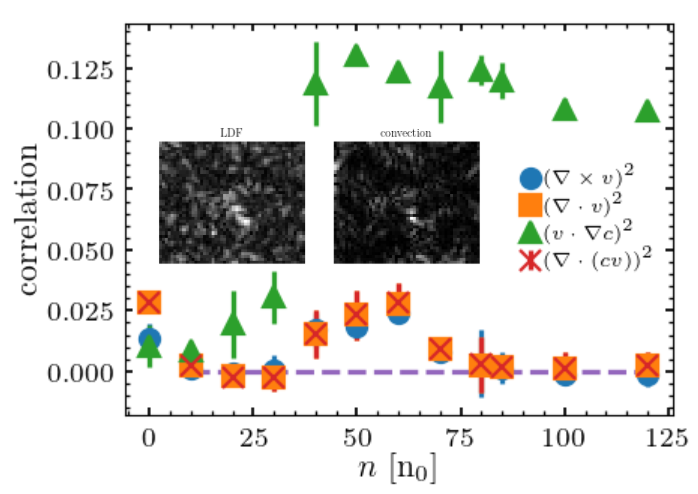
\includegraphics[width=0.8\textwidth]{GNF_figure-5-v1.png}
\caption[]{Correlations between local number fluctuations and flow fields. Insets show the local density fluctuation field and convection field at steady state in a 80 n$_0$ bacterial suspension. }
\label{fig:5}
\end{center}
\end{figure*}

\section{Conclusions}


\section*{Acknowledgments}

\bibliographystyle{apsrev4-2}
%\bibliography{cracks}
\bibliography{correlations}



\end{document}
